\begin{frame}
	\frametitle{Software Diversity}

	Study of diversity in software and software engineering

	\vspace{0.5cm}

	E.g web browsers, database management systems, compilers (GCC or Clang) etc

\end{frame}

\begin{frame}
	\frametitle{Why Software Diversity?}

	\begin{itemize}
		\item Security
			\begin{itemize}
				\item	Address Space Layout Randomization
			\end{itemize}
		\item Testing
			\begin{itemize}
				\item Generate diverse test cases
			\end{itemize}
		\item	Fault-tolerance/Error-handling
			\begin{itemize}
				\item N-versioning\cite{n-version}
			\end{itemize}
	\end{itemize}

\end{frame}

\begin{frame}
	\frametitle{Automated Sofware Divesity}

	Only devise the process.

	\vspace{0.5cm}

	Static diversity; Generate a diverse population of executables at compile time.

	\vspace{0.5cm}

	Dynamic diversity; Generate one executable that provides diverse run-times.

\end{frame}

\begin{frame}
	\frametitle{Code re-use attacks}

	Divert the NX bit

	\vspace{0.5cm}

	Hijacking control flow

	\vspace{0.5cm}

	Execute already loaded code in an unintended manner

\end{frame}

\begin{frame}
	\frametitle{Example of code re-use attack}

	\begin{itemize}
		\item Challenge on ROP Emporium (https://ropemporium.com/)
		\item One executable, split, and a file called "flag.txt"
		\item Make split execute system("/bin/cat flag.txt")
			\begin{itemize}
				\item x86-64
				\item Linux
			\end{itemize}
	\end{itemize}

	\vspace{0.5cm}

	\begin{itemize}
		\item	Buffer Overflow vulnerability
		\item All puzzle pieces are present
		\item	Find an instruction sequence that allows us to set up the arguments
		\item	Overwrite the return address on the stack to hijack control flow
	\end{itemize}

\end{frame}

% Frame with picture
\begin{frame}
	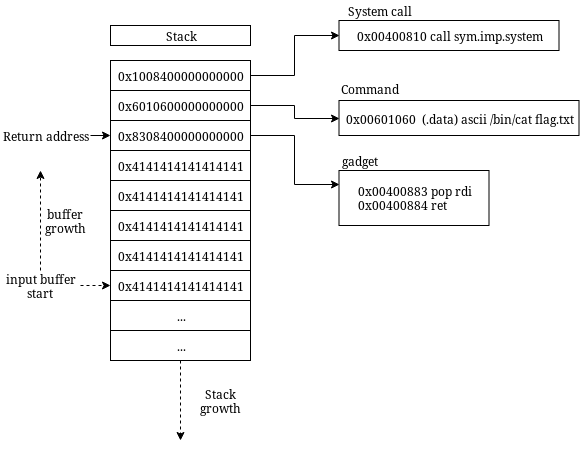
\includegraphics[width=\textwidth]{../background/software-diversity/figures/after-payload}
\end{frame}

\begin{frame}
	\frametitle{Return Oriented Programming}

	The instruction sequences are dubbed \textit{gadgets}.

	\vspace{0.5cm}

	Not only for setting up arguments. Can be chained together to perform arbitrary operations.

	\vspace{0.5cm}

	Introduced on x86, where they are frequent.

\end{frame}

\begin{frame}
	\frametitle{Defenses}

	Payload relies on the exact addresses of the gadgets

	\vspace{0.5cm}

	Compilers make many decisions, not all are the only valid one

	\vspace{0.5cm}

	Many solutions today introduce chance somewhere in the process

	\vspace{0.5cm}

	Systematically explore the combinations of decisions and generate a population of executables.

	\begin{itemize}
		\item Guarantess about population
		\item Correctness of transformation
		\item Fine-grained control of process
	\end{itemize}

\end{frame}
